\documentclass{article}[12pt]
\usepackage[a4paper, margin=1in]{geometry}
\usepackage[utf8]{inputenc}
\usepackage[english]{babel}
\usepackage{amssymb, amsmath, amsthm} % math symbols
\usepackage{hyperref} % hyperlinks
\usepackage[table]{xcolor} % tables
\usepackage{graphicx}

\hypersetup{
    colorlinks=true,
    linkcolor=black,
    citecolor=black,
    urlcolor=blue,
    pdfborderstyle={/S/U/W 1}
    }

% title
\title{Learning Notation: Seminar Three \\ Differential Calculus}
\author{Jack (Quan Cheng) Xie}
\date{\today}
    
% paragraph /indent spacing
\setlength{\parskip}{6pt}
\setlength{\parindent}{0pt}

% mathtools equation numbering
\counterwithin*{equation}{section}
\renewcommand\theequation{\thesection.\arabic{equation}}

% amsthm theorems formatting
\newtheorem{theorem}{Theorem}

\newtheorem{conjecture}{Conjecture}

\newtheorem{proposition}{Proposition}

\newtheorem{definition}{Definition}

\newtheorem{paradox}{Paradox}

\newtheorem{exercise}{Exercise}

% special symbols
\newcommand{\N}{\mathbb{N}}
\newcommand{\Z}{\mathbb{Z}}
\newcommand{\Q}{\mathbb{Q}}
\newcommand{\R}{\mathbb{R}}
\newcommand{\C}{\mathbb{C}}
\newcommand{\PS}{\mathcal{P}}

% text box for definitions and theorems
\newcommand{\textbox}[1]{\fbox{\parbox{\textwidth}{#1}}}

% bibliography formatting
\makeatletter
\renewcommand{\@biblabel}[1]{$\triangleright$}
\makeatother

% Resources
% https://www.youtube.com/watch?v=RjPXfUT7Odo
% https://www.youtube.com/watch?v=Q9KOeP-nrYQ

\begin{document}

    \maketitle
    
    \section{Limits of Functions}
    % Epsilon-delta definition
    
    \subsection{Definitions and continuity}
    
        For a first look at limits in calculus, we often use a more intuitive, informal definition. 
        
        \textbox{
        \begin{definition}[Informal]
            The limit of a function $f(x)$ equals $L$ as $x$ approaches $p$, written as
            \begin{align}
                \lim_{x \to p} f(x) = L,
            \end{align}
            if $f(x)$ gets arbitrarily close to $L$ as $x$ gets arbitrarily close to $p$, or \begin{align}
                f(x) \to L \text{ as } x \to p.
            \end{align}
        \end{definition}
        }
    
        However, this informal definition is a little too fuzzy. For instance, what $x \to p$ means is not really defined. We need a more rigorous definition to derive proofs about limits and other calculus results. The standard in real analysis is the \textbf{epsilon-delta definition}.
        
        \textbox{
        \begin{definition}[Epsilon-delta]
            For any real function $f(x)$, we say its \textbf{limit} equals $L$ as $x$ approaches a \textbf{limit point} $p$, and write
            \begin{align}
                \lim_{x \to p} f(x) = L,
            \end{align}
            if for every $\varepsilon \in \R^+$, there exists $\delta \in \R^+$ such that for all $x \in \R$,
            \begin{align}
                | x - p | < \delta
                \implies
                | f(x) - L | < \varepsilon.
            \end{align}
        \end{definition}
        }
        
        Essentially this definition is the same as our informal one, but structured much more precisely. 
        
        See Figure \ref{fig:epsilon-delta} for an geometric illustration of the definition. Note that $|y - c| < k \iff y - k < c < k + y$. This can be proven by cases, when $y - c$ is positive and negative.
        
        \begin{figure}[!ht]
            \centering
            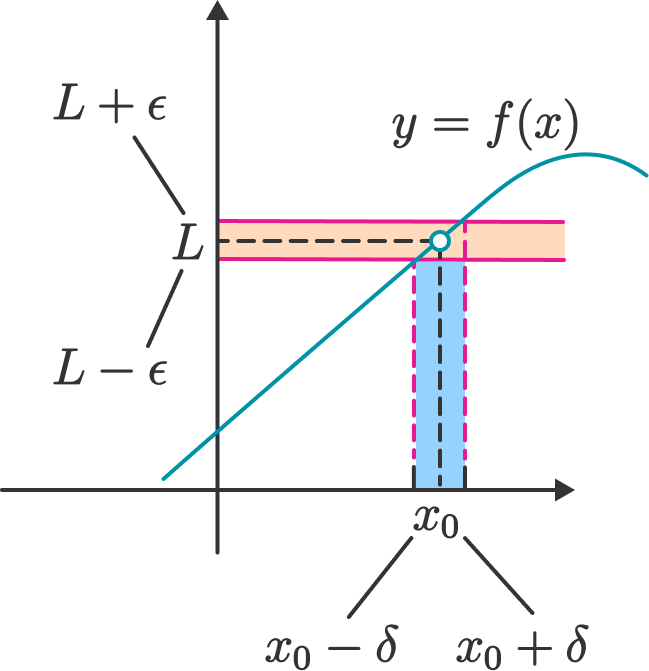
\includegraphics[width=0.45\textwidth]{attachments/3.1-limit.png}
            \caption{From \href{https://brilliant.org/wiki/epsilon-delta-definition-of-a-limit/}{brilliant.org}. Here $x_0$ is the limiting point we defined as $p$.}
            \label{fig:epsilon-delta}
        \end{figure}
        
        \textbox{
        \begin{definition}[Continuity]
            A real function $f(x)$ is \textbf{continuous} at $p$ if
            \begin{align}
                \lim_{x \to p} f(x) = f(p).
            \end{align}
            Otherwise $f(x)$ is \textbf{discontinuous} at $p$.
        \end{definition}
        }
    
        For limits at infinity and certain discontinuous points, it is useful also to define one-sided limits using similar epsilon-delta definitions.
        
        \textbox{
        \begin{definition}[Limit from below]
            The limit of $f(x)$ \textbf{from above} as $x$ approaches $p$ is equal to $L$, written as
            \begin{align}
                \lim_{x \to p^+} f(x) = L
                \quad\text{or}\quad
                \lim_{x \downarrow p} f(x) = L,
            \end{align}
            if for every $\epsilon \in \R^+$, there exists $\delta \in \R^+$ such that
            \begin{align}
                0 < x - p < \delta
                \implies
                |f(x) - L| < \varepsilon.
            \end{align}
            
            We define limits as $x$ approaches negative infinity as the limit from above,
            \begin{align}
                \lim_{x \to -\infty} f(x) = \lim_{x \downarrow -\infty} f(x),
            \end{align}
            where $\forall x \in \R, \ x > -\infty$.
        \end{definition}
        }
            
        \textbox{
        \begin{definition}[Limit from above]
            Similarly, the limit of $f(x)$ \textbf{from below} as $x$ approaches $p$ is equal to $L$, written as
            \begin{align}
                \lim_{x \to p^-} f(x) = L
                \quad\text{or}\quad
                \lim_{x \uparrow p} f(x) = L,
            \end{align}
            if for every $\epsilon \in \R^+$, there exists $\delta \in \R^+$ such that
            \begin{align}
                0 < p - x < \delta
                \implies
                |f(x) - L| < \varepsilon.
            \end{align}
            
            We define limits as $x$ approaches positive infinity as the limit from below,
            \begin{align}
                \lim_{x \to \infty} f(x) = \lim_{x \uparrow \infty} f(x),
            \end{align}
            where $\forall x \in \R, \ x < \infty$.
        \end{definition}
        }
        
        These one-sided definitions now give us sensible consequences of taking limits at positive and negative infinity. We can also use one-sided limits to check for the existence of the limit and therefore continuity.
        
        % \begin{exercise}
        %     Show from the epsilon-delta definitions that
        %     \begin{align}
        %         \lim_{x\to \infty} \frac{1}{x} = 0
        %     \end{align}
        % \end{exercise}
        
        \begin{exercise}
            Prove that
            \begin{align}
                \lim_{x\to p} f(x)
                = L
                \iff
                \lim_{x \to p^-} f(x)
                = \lim_{x \to p^+} f(x)
                = L.
            \end{align}
        \end{exercise}
        
        % \begin{exercise}
        %     Show that if
        %     \begin{align}
        %         \lim_{x \to p^-} f(x) \ne
        %         \lim_{x \to p^+} f(x),
        %     \end{align}
        %     then $f(x)$ is discontinuous at $p$.
        % \end{exercise}
        
        
    \subsection{Properties of limits}
    
    
    \section{Differentiation}

        Now that we have defined limits and know some of their properties, we can define differentiation and derive their properties also.  
        
        \textbox{
        \begin{definition}[Derivative]
            The derivative of a function $f(x)$, written as $f'(x)$, is defined as the limit
            \begin{align}
                f'(x) = \lim_{h \to 0}\frac{f(x+h) - f(x)}{h}.
            \end{align}
        \end{definition}
        }
        
        % Differentiability
        
        % Derivative rules proofs
        
        % Logarithms and exponentiation
    
    \section{Multivariable Derivatives}
    
    % Gradient vector
    
    % Hessian matrix
    
    % Positive/negative-definite matrix
    
    \section{Optimization}
    
    % Convex sets
    
    % Concave and concave functions
    
    % First and second-order conditions for local extreme points
    
    % Lagrange multipliers
    
        % https://ocw.mit.edu/courses/mathematics/18-02sc-multivariable-calculus-fall-2010/2.-partial-derivatives/part-c-lagrange-multipliers-and-constrained-differentials/session-40-proof-of-lagrange-multipliers/MIT18_02SC_notes_22.pdf
    
    % Kuhn-Tucker Conditions
        % Hyperplane separation theorem
    
    % Envelope theorem
    
\end{document}